\subsection{Nono sprint}

\begin{minipage}{\textwidth}
  Di seguito è riportata la distribuzione delle ore per ciascun membro del team, accumulate in totali per persona e per ruolo:
  \begin{table}[H]
    \begin{tabularx}{\textwidth}{|c|*{6}{>{\centering}X|}c|}
      \hline
      \multicolumn{8}{|c|}{\textbf{Consuntivo orario}} \\
      \hline
      \textbf{Membro del team} & \textbf{Re} & \textbf{Am} & \textbf{An} & \textbf{Pt} & \textbf{Pr} & \textbf{Ve} & \textbf{Totale per persona} \\
      \hline
      Cavalli Riccardo & 0 & 0 & 0 & 2 & 1 & 2 & 5 \\
      \hline
      Pianon Raul & 0 & 2 & 0 & 1 & 0 & 1 & 4 \\
      \hline
      Dall’Amico Martina & 1 & 0 & 0 & 0 & 0 & 3 & 4 \\
      \hline
      Cristo Marco & 0 & 2 & 0 & 0 & 0 & 2 & 4 \\
      \hline
      Lewental Sebastiano & 2 & 0 & 0 & 0 & 0 & 2 & 4 \\
      \hline
      Zecchinato Mattia & 0 & 0 & 0 & 2 & 0 & 2 & 4 \\
      \hline
      Stocco Tommaso & 0 & 0 & 0 & 0 & 1 & 3 & 4 \\
      \hline
      \textbf{Totale ore per ruolo} & 3 & 4 & 0 & 6 & 1 & 15 & \textbf{29} \\
      \hline
    \end{tabularx}
    \caption{Sprint 9 - Consuntivo orario}
  \end{table}
  \end{minipage}

  % \begin{figure}[H]
  %   \centering
  %   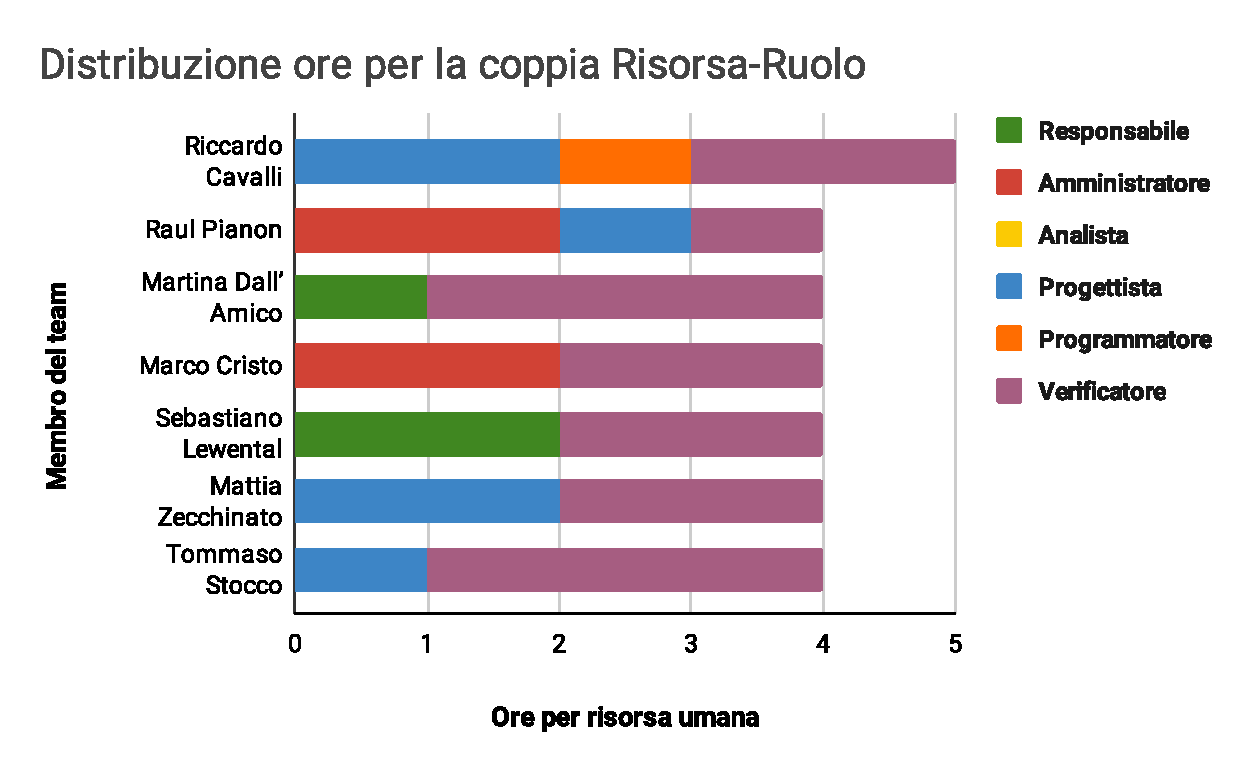
\includegraphics[width=0.90\textwidth]{assets/Consuntivo/Sprint-9/distribuzione_ore_risorsa_ruolo.pdf}
  %   \caption{Sprint 9 - Istogramma della distribuzione oraria per la coppia risorsa-ruolo}
  % \end{figure}

  % \begin{figure}[H]
  %   \centering
  %   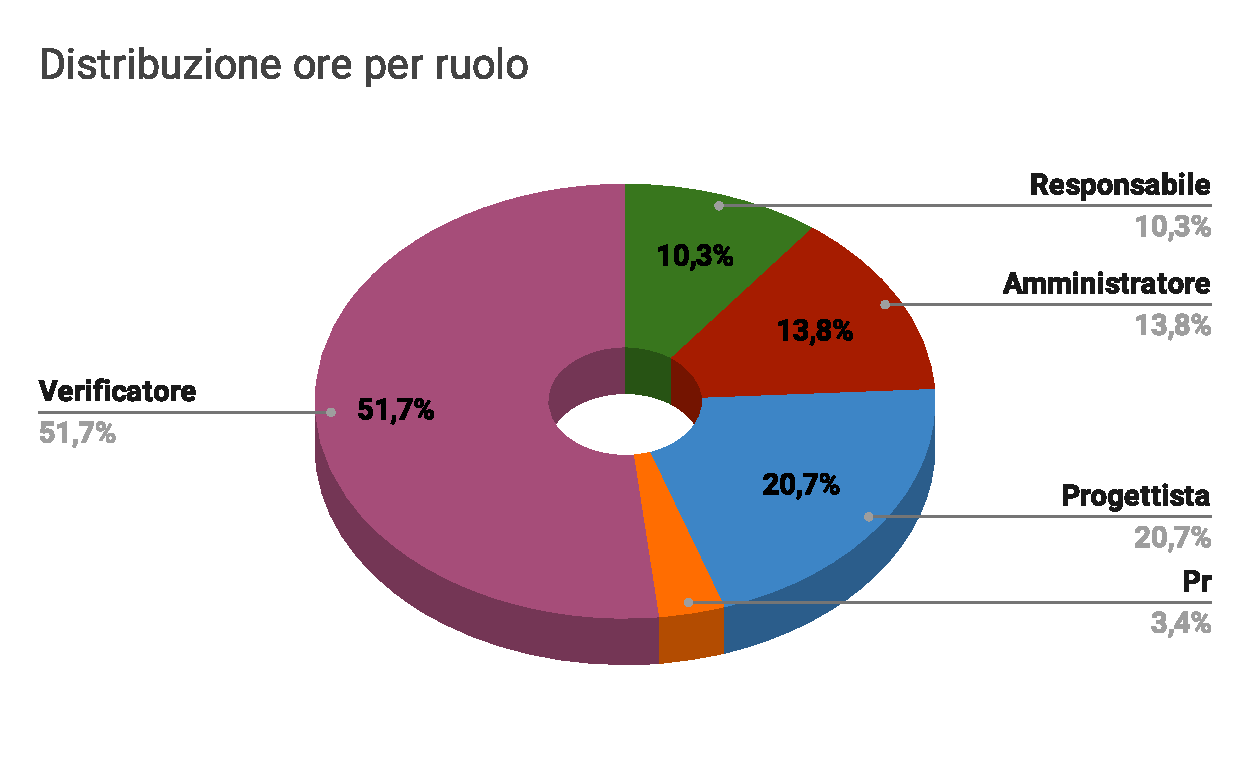
\includegraphics[width=0.90\textwidth]{assets/Consuntivo/Sprint-9/distribuzione_ore_ruolo.pdf}
  %   \caption{Sprint 9 - Areogramma della distribuzione oraria per ruolo}
  % \end{figure}

  \begin{minipage}{\textwidth}
  Di seguito è riportato il consuntivo economico del nono \glossario{sprint}:
  \begin{table}[H]
  \begin{adjustwidth}{-0.5cm}{-0.5cm}
    \centering
    \begin{tabular}{|P{2.9cm}|P{2.3cm}|P{2.5cm}|P{2.3cm}|>{\arraybackslash}P{2.5cm}|}
      \hline
      \multicolumn{5}{|c|}{\textbf{Consuntivo economico}} \\
      \hline
      \textbf{Ruolo} & \textbf{Ore per ruolo} & \textbf{Delta ore preventivo - consuntivo} & \textbf{Costo (in \texteuro)} & \textbf{Delta costo preventivo - consuntivo (in \texteuro)} \\
      \hline
      Responsabile & 3 & 0 & 90,00 & 0,00 \\ \hline
      Amministratore & 4 & 0 & 80,00 & 0,00 \\ \hline
      Analista & 0 & 0 & 0,00 & 0,00 \\ \hline
      Progettista & 6 & -1 & 150,00 & -25,00 \\ \hline
      Programmatore & 1 & 0 & 15,00 & 0,00 \\ \hline
      Verificatore & 15 & 0 & 225,00 & 0,00 \\ \hline
      \textbf{Totale} & \textbf{29} & -1 & \textbf{560,00} & -25,00 \\ \hline
      \textbf{Restante} & 296 & / & 5.940,00 & / \\ \hline
      \textbf{Sprint pregressi} & 321 & / & 6.520,00 & / \\ \hline
    \end{tabular}
    \caption{Sprint 9 - Consuntivo economico}
  \end{adjustwidth}
  \end{table}
  \end{minipage}

  % \begin{figure}[H]
  %   \centering
  %   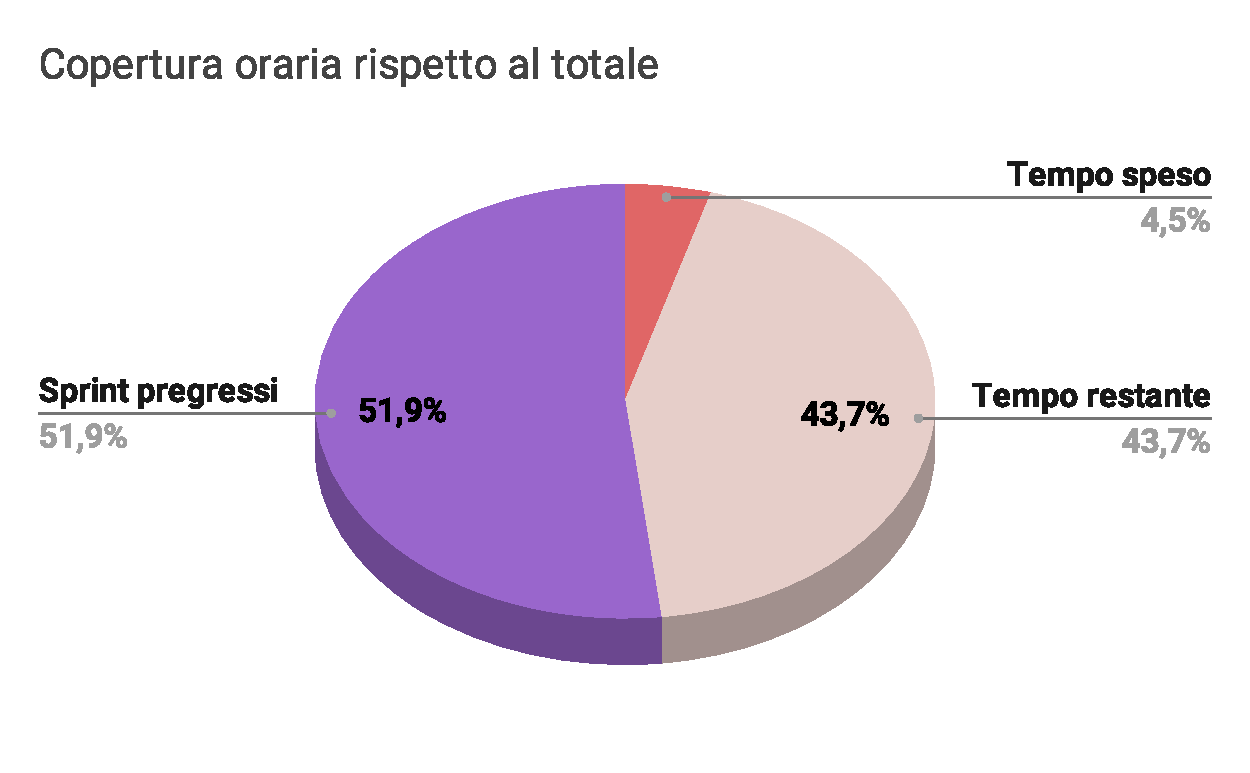
\includegraphics[width=0.90\textwidth]{assets/Consuntivo/Sprint-9/copertura_oraria.pdf}
  %   \caption{Sprint 9 - Areogramma del tempo speso (in ore) rispetto al totale}
  % \end{figure}

  % \begin{figure}[H]
  %   \centering
  %   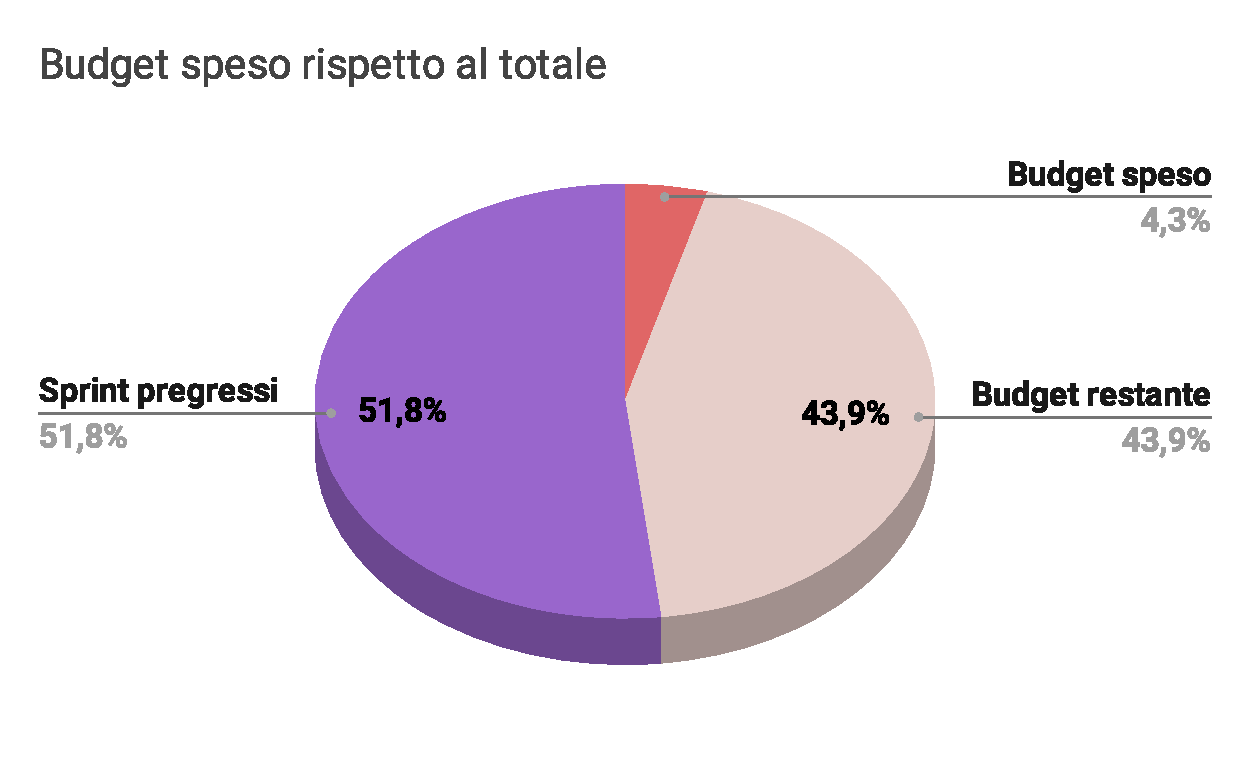
\includegraphics[width=0.90\textwidth]{assets/Consuntivo/Sprint-9/budget_speso.pdf}
  %   \caption{Sprint 9 - Areogramma del budget speso rispetto al totale}
  % \end{figure}

  \begin{minipage}{\textwidth}
    Di seguito sono riportate le ore rimanenti per la coppia risorsa-ruolo:
    \begin{table}[H]
      \begin{tabularx}{\textwidth}{|c|*{6}{>{\centering}X|}c|}
        \hline
        \multicolumn{8}{|c|}{\textbf{Ore rimanenti per la coppia risorsa-ruolo}} \\
        \hline
        \textbf{Membro del team} & \textbf{Re} & \textbf{Am} & \textbf{An} & \textbf{Pt} & \textbf{Pr} & \textbf{Ve} & \textbf{Totale per persona} \\
        \hline
        Cavalli Riccardo & 0 & 0 & 4 & 12 & 10 & 9 & 35 \\
        \hline
        Pianon Raul & 2 & 1 & 1 & 19 & 9 & 8 & 40 \\
        \hline
        Dall’Amico Martina & 2 & 1 & 1 & 14 & 16 & 812 & 42 \\
        \hline
        Cristo Marco & 2 & 4 & 1 & 17 & 10 & 8 & 42 \\
        \hline
        Lewental Sebastiano & 3 & 4 & 1 & 11 & 14 & 10 & 43 \\
        \hline
        Zecchinato Mattia & 5 & 2 & 3 & 9 & 13 & 12 & 44 \\
        \hline
        Stocco Tommaso & 5 & 0 & 3 & 19 & 9 & 12 & 48 \\
        \hline
        \textbf{Totale ore per ruolo} & 19 & 13 & 14 & 101 & 82 & 67 & \textbf{296} \\
        \hline
      \end{tabularx}
      \caption{Sprint 9 - Ore rimanenti per la coppia risorsa-ruolo}
    \end{table}
  \end{minipage}

\subsubsection{Revisione delle attività}

Nell'arco del nono \glossario{sprint}, il team ha svolto le seguenti attività:
\begin{itemize}
  \item Test su database locale;
  \item Aggiornamento delle \NdP;
  \item Estensione sezioni delle \NdP;
  \item Stesura iniziale del documento di Specifiche Tecniche;
  \item Aggiornamento del \PdP;
  \item Revisione delle \NdP;
  \item Revisione del \PdP;
  \item Stesura e aggiornamento dei verbali interni;
\end{itemize}

\subsubsection{Retrospettiva}

\par Di seguito sono riportati i risultati del questionario di valutazione dello \glossario{sprint}:
\begin{itemize}
  \item Organizzazione dello \glossario{sprint}\ - Valutazione: 8;
  \item Conduzione dei meeting interni - Valutazione: 8;
  \item Conduzione dei meeting esterni - Valutazione: 8;
  \item Impegno e partecipazione dei singoli membri - Valutazione: 2.5;
  \item Tutti i membri del gruppo sapevano cosa fare nel loro ruolo;
  \item La numerosità delle riunioni è risultata adeguata per quasi tutti i membri del gruppo;
  \item Le riunioni sono state organizzate sempre con il giusto preavviso;
  \item Il rapporto ore spese/ore produttive è sbilanciato a causa della sessione d'esami;
  \item La produttività è stata comunque ragionevole considerando le criticità della sessione;
\end{itemize}

\vspace{0.5\baselineskip}
\par A seguire le \textbf{analisi a posteriori} del nono \glossario{sprint}:
\begin{itemize}
  \item Durante questo \glossario{sprint} il team si è concentrato sul completamento delle attività mancanti in vista dell'incontro con il Professor Riccardo Cardin per la revisione \RTB. Dal prossimo \glossario{sprint}, il gruppo si concentrerà sulla conclusione delle attività rimaste per il completamento della documentazione in vista della seconda parte della revisione. In seguito a ciò, si inizieranno anche i lavori per la progettazione logica e architetturale del prodotto.
  \item La sessione d'esami ha impattato notevolmente sulla quantità di lavoro svolto, come previsto. 
\end{itemize}

\subsubsection{Aggiornamento pianificazione e preventivo}
\par Il team ha definito un piano d'azione per migliorare l'organizzazione e la produttività del prossimo \glossario{sprint}:
\begin{itemize}
  \item Il team ha optato per l'organizzazione di \glossario{sprint} della durata di due settimane.
\end{itemize}

\paragraph*{Pianificazione futura:}
\par Conclusa la fase di \RTB e terminata la sessione estiva d'esami, il gruppo ha deciso di tornare alla programmazione di \glossario{sprint} di due settimane, così da favorire un progresso più flessibile e meno restrittivo: in questo modo sarà possibile incentrare un maggiore focus sulla progettazione, garantendo comunque il tempo necessario per un'accurata e completa redazione della documentazione.

\paragraph*{Preventivo "a finire" (\sezione{sec:stima_temporale}):}
\par Effettuata la prima presentazione della revisione RTB, il gruppo rimane in attesa dell'esito da parte della Committente, preparando nel frattempo la documentazione necessaria ad affrontare la seconda fase PB. Si mantiene un carico di lavoro equilibrato, tenendo sempre in considerazione il periodo corrente di sessione d'esami.

\paragraph*{Gestione dei rischi (\sezione{sec:analisi_rischi}):}
\par Nel corso del nono \glossario{sprint}, il seguente rischio si è presentato ed è stato gestito correttamente:
\begin{itemize}
  \item \textbf{Rischi relativi a rallentamenti}: Durante la sessione di esami, le ore di lavoro assegnate a ciascun membro sono state calcolate in concomitanza con le ore di studio individuale; poiché questo rischio era stato previsto, la data di consegna era stata pianificata di conseguenza, non comportando quindi disguidi operativi.
\end{itemize}

\vspace{0.5\baselineskip}
\par Durante il nono \glossario{sprint}, alcune contromisure si sono rivelate utili a mitigare i rischi individuati in fase di pianificazione. In particolare:
\begin{itemize}
  \item Corretta organizzazione preventiva.
\end{itemize}
